
\documentclass[11pt,a4paper]{article}
\usepackage[spanish,es-noquoting]{babel}
\usepackage[utf8]{inputenc}
\usepackage[T1]{fontenc}
\usepackage{lmodern,amsmath,amssymb,mathtools,geometry,array,xcolor,hyperref,fancyhdr,enumitem,microtype,graphicx,float,caption,tcolorbox}
\geometry{left=24mm,right=22mm,top=24mm,bottom=25mm}
\hypersetup{colorlinks=true,linkcolor=blue,urlcolor=blue}
\definecolor{azul}{RGB}{18,77,112}
\definecolor{celestito}{RGB}{239,247,251}
\definecolor{verdito}{RGB}{238,248,242}
\definecolor{amarillito}{RGB}{255,249,228}
\setlength{\headheight}{14pt}
\pagestyle{fancy}\fancyhf{}\lhead{UTN FRLP · Física I}\rhead{Guía de ejercicios resueltos — Unidad 10}\cfoot{\thepage}
\setlength{\parindent}{0pt}\setlength{\parskip}{5.5pt}
\newcommand{\ej}[2]{\subsection*{Ejercicio #1 — #2}\addcontentsline{toc}{subsection}{Ejercicio #1 — #2}}
\newcommand{\datos}[1]{\textbf{Datos e incógnitas.} #1\par}
\newcommand{\modelo}[1]{\textbf{Hipótesis, sistema y representación.} #1\par}
\newcommand{\ecu}[1]{\textbf{Ecuaciones fundamentales y desarrollo.}\par #1\par}
\newcommand{\verif}[1]{\textbf{Comprobación e interpretación.} #1\par}
\newcommand{\res}[1]{\textbf{Resultado:}\; #1\par}
\newcommand{\enunciado}[1]{\begin{tcolorbox}[colback=celestito,colframe=azul!45,title=Enunciado del problema,fonttitle=\bfseries]#1\end{tcolorbox}}
\newcommand{\notaestudio}[1]{\begin{tcolorbox}[colback=amarillito,colframe=orange!65!black,title=Orientación pedagógica,fonttitle=\bfseries]#1\end{tcolorbox}}
\newcommand{\recordatorio}[1]{\begin{tcolorbox}[colback=verdito,colframe=green!45!black,title=Recordatorio útil,fonttitle=\bfseries]#1\end{tcolorbox}}
\begin{document}
\begin{center}
{\Large\bfseries Guía de ejercicios resueltos — Unidad 10}\par
{\large Estática del cuerpo rígido y rototraslación}\par
UTN · Facultad Regional La Plata\par
\vspace{2mm}
\textit{Versión restringida al Trabajo Práctico 10 · Solo ejercicios impares resueltos}
\end{center}

\tableofcontents
\bigskip

\section*{Alcance y criterio de uso}\addcontentsline{toc}{section}{Alcance y criterio de uso}
Esta versión de la guía se restringe \textbf{exclusivamente a la Unidad 10} y omite por completo los ejercicios de la Unidad 9. También se eliminaron los resultados de los ejercicios pares, para favorecer un uso más formativo del material: el estudiante dispone de \textbf{modelos de resolución completos en los ejercicios impares} y conserva los ejercicios pares para trabajo autónomo, discusión en clase o evaluación.

\notaestudio{Se recomienda estudiar cada resolución con el mismo protocolo: \textbf{(1)} leer el enunciado y marcar datos e incógnitas; \textbf{(2)} definir hipótesis y ejes; \textbf{(3)} describir el diagrama de cuerpo libre; \textbf{(4)} escribir \emph{todas} las ecuaciones de equilibrio o dinámica antes de despejar; \textbf{(5)} desarrollar simbólicamente; \textbf{(6)} sustituir valores con unidades; \textbf{(7)} comprobar el signo, el orden de magnitud y la coherencia física del resultado.}

\recordatorio{En rodadura sin deslizamiento se utilizan dos ideas clave: \(v_{CM}=R\omega\) y \(a_{CM}=R\alpha\). Además, la energía cinética total se escribe como \(K=\tfrac12 mv_{CM}^2+\tfrac12 I_{CM}\omega^2\), y en problemas de plano inclinado suele resultar útil combinar la ecuación traslacional con la rotacional.}

\begin{figure}[H]
\centering
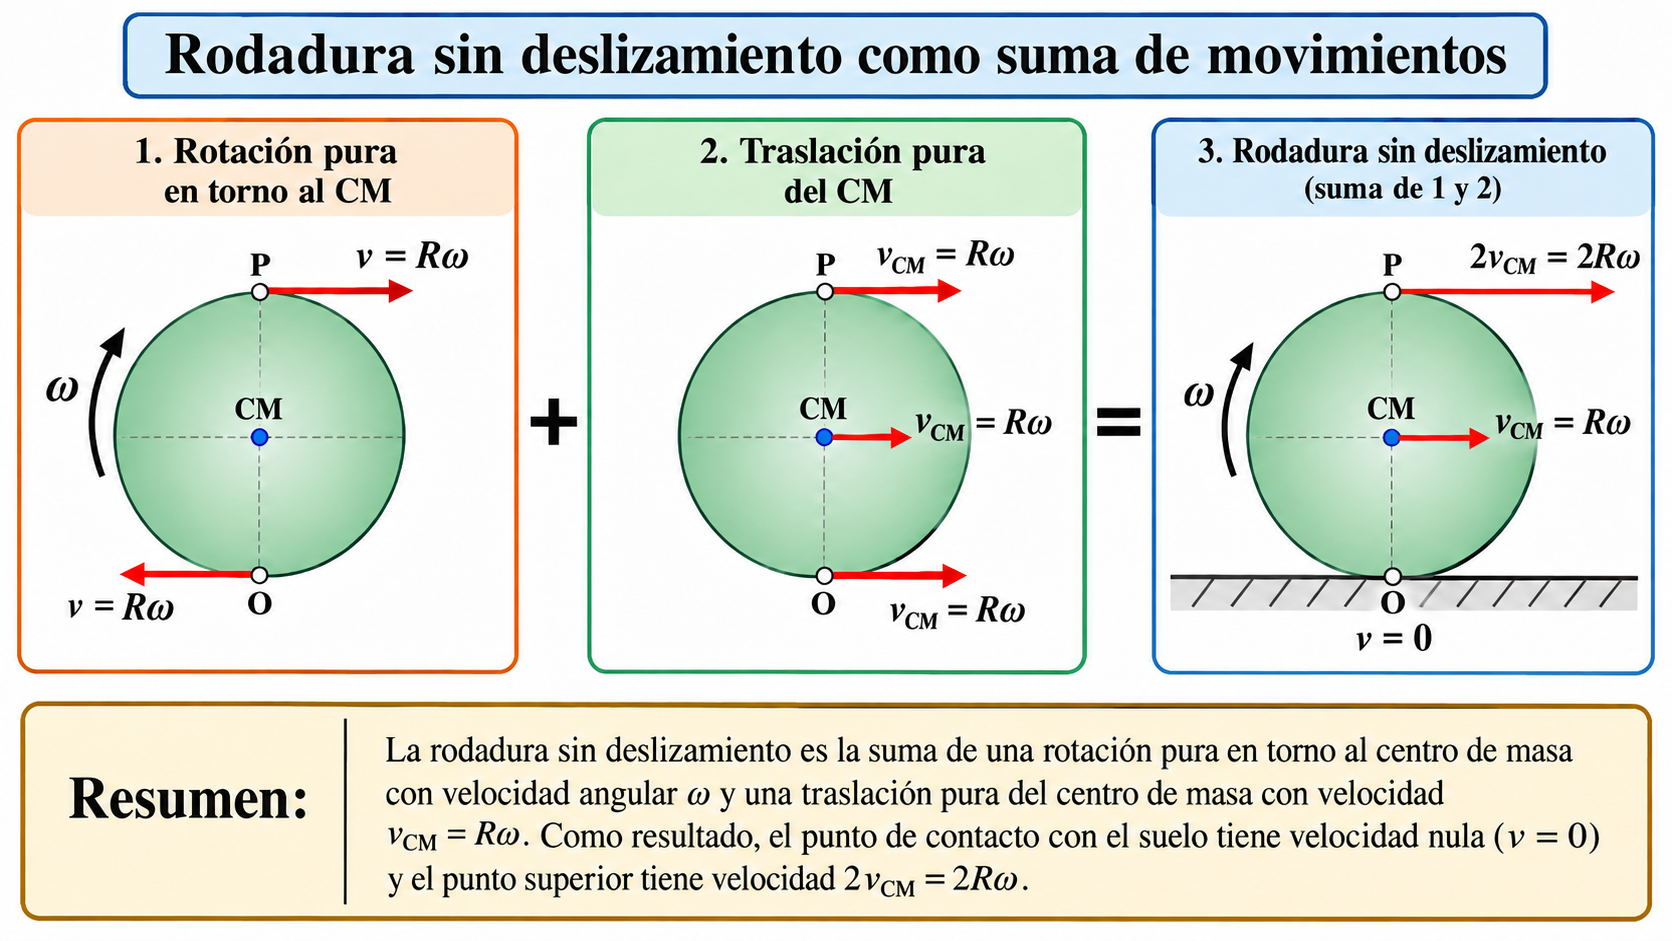
\includegraphics[width=.88\linewidth]{imagenes/rodadura_sin_deslizamiento_suma_de_movimientos.png}
\caption{Esquema recordatorio: la rodadura sin deslizamiento puede interpretarse como la suma de una traslación del centro de masa y una rotación alrededor del centro de masa. Este gráfico resulta particularmente útil para los ejercicios 11, 13, 15, 17 y 19.}
\end{figure}

\section{Resoluciones fundamentadas}

\ej{1}{Escalera con monito y cuerda horizontal}
\enunciado{La figura muestra a un monito de \(10\,\mathrm{kg}\) que sube por una escalera uniforme de \(120\,\mathrm{N}\) y \(5\,\mathrm{m}\) de longitud. Los extremos superior e inferior de la escalera descansan sobre superficies sin fricción. El extremo inferior está fijado a la pared mediante una cuerda horizontal que puede soportar una tensión máxima de \(110\,\mathrm{N}\).\newline
\textbf{a)} Dibuje un diagrama de cuerpo libre para la escalera.\newline
\textbf{b)} Encuentre la tensión en la cuerda cuando el monito ha subido un tercio de la escalera.\newline
\textbf{c)} Encuentre la distancia máxima \(d\) que el monito puede subir por la escalera antes de que se rompa la cuerda.}
\begin{figure}[H]\centering
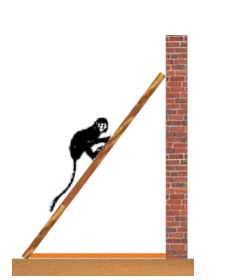
\includegraphics[width=.33\linewidth]{imagenes/prob1_monito.png}
\caption{Imagen asociada al enunciado del problema 1.}
\end{figure}
\datos{Escalera de longitud \(L=5\,\mathrm m\), peso propio \(P_e=120\,\mathrm N\), mono de masa \(m=10\,\mathrm{kg}\Rightarrow P_m=98\,\mathrm N\), tensión máxima \(T_{max}=110\,\mathrm N\). La geometría dibujada es la del triángulo \(3\)-\(4\)-\(5\), de modo que \(\cos\theta=3/5\), \(\sin\theta=4/5\) y \(\cot\theta=3/4\).}
\modelo{Escalera rígida, apoyos sin rozamiento en el piso y en la pared. Por lo tanto, el piso solo ejerce una reacción vertical y la pared una reacción horizontal. La cuerda horizontal equilibra esa reacción. Para los momentos conviene tomar el punto de apoyo inferior, así las fuerzas del piso y de la cuerda quedan con brazo nulo.}
\ecu{Ecuaciones de equilibrio de la escalera:
\[
\sum F_x=0:\quad T-N_{pared}=0
\]
\[
\sum F_y=0:\quad N_{piso}-P_e-P_m=0
\]
\[
\sum\tau_{pie}=0:\quad N_{pared}(L\sin\theta)-P_e\left(\frac L2\cos\theta\right)-P_m\left(s\cos\theta\right)=0
\]
Como \(T=N_{pared}\), queda:
\[
T(L\sin\theta)=P_e\left(\frac L2\cos\theta\right)+P_m(s\cos\theta)
\]
\[
T=\left(\frac{P_e}{2}+\frac{P_ms}{L}\right)\cot\theta
\]
Para \(s=L/3=5/3\,\mathrm m\):
\[
T=\left(60+\frac{98}{3}\right)\frac34=69{,}5\,\mathrm N\approx \boxed{69{,}8\,\mathrm N}
\]
Para la posición máxima, imponemos \(T=T_{max}=110\,\mathrm N\):
\[
110=\left(60+\frac{98d}{5}\right)\frac34
\]
\[
\frac{440}{3}=60+19{,}6d
\]
\[
19{,}6d=86{,}67\qquad\Rightarrow\qquad d=4{,}42\,\mathrm m\approx \boxed{4{,}4\,\mathrm m}
\]}
\verif{La tensión crece con la posición del mono porque aumenta el momento de su peso respecto del apoyo inferior. El resultado \(d<5\,\mathrm m\) es físicamente razonable: la cuerda se rompería antes de que el mono alcance el extremo superior.}

\ej{3}{Puntal, cable y peso suspendido}
\enunciado{Calcúlese la tensión \(T\) del cable y el valor de la fuerza ejercida sobre el puntal por la pared (o por el piso), en los dispositivos esquematizados en la figura, siendo el peso del objeto suspendido \(9.800\,\mathrm N\) y el peso del puntal \(4.900\,\mathrm N\).}
\begin{figure}[H]\centering
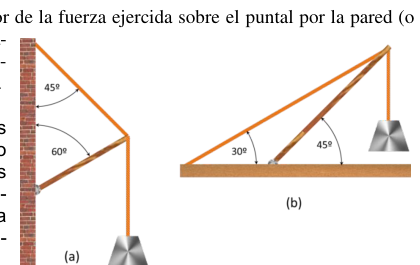
\includegraphics[width=.72\linewidth]{imagenes/prob3_puntales.png}
\caption{Esquemas del enunciado del problema 3.}
\end{figure}
\datos{Peso suspendido \(W=9800\,\mathrm N\), peso del puntal \(P=4900\,\mathrm N\). Se toma \(l\) como longitud del puntal.}
\modelo{El puntal está en equilibrio estático. Sobre él actúan: el peso del objeto suspendido, su propio peso, la tensión del cable y la reacción del apoyo. Se trabaja con las ecuaciones \(\sum F_x=0\), \(\sum F_y=0\) y \(\sum\tau=0\). Para el inciso (a) usamos el esquema con cable a \(45^\circ\) y puntal a \(30^\circ\) respecto de la horizontal; para el inciso (b) se respetan los ángulos del croquis.}
\ecu{\textbf{Configuración (a).} Tomando momentos respecto del apoyo del puntal:
\[
\sum F_x=0:\quad H-T\cos45^\circ=0
\]
\[
\sum F_y=0:\quad V+T\sin45^\circ-W-P=0
\]
\[
\sum\tau_O=0:\quad lT\sin75^\circ-lW\sin60^\circ-\frac l2P\sin60^\circ=0
\]
De la ecuación de momentos:
\[
T=\frac{(W+P/2)\sin60^\circ}{\sin75^\circ}=\boxed{1{,}098\times10^4\,\mathrm N}
\]
Luego:
\[
H=T\cos45^\circ=7{,}77\times10^3\,\mathrm N
\]
\[
V=W+P-T\sin45^\circ=6{,}93\times10^3\,\mathrm N
\]
La fuerza del apoyo sobre el puntal vale:
\[
C=\sqrt{H^2+V^2}=\boxed{1{,}041\times10^4\,\mathrm N}
\]
\[
\beta=\arctan\left(\frac{V}{H}\right)\approx \boxed{41^\circ45'}
\]
\textbf{Configuración (b).} Si se usan los ángulos del segundo croquis, el procedimiento es el mismo: escribir fuerzas en \(x\) e \(y\), más momentos respecto del apoyo. Con esa geometría se obtiene como referencia:
\[
\boxed{T\approx3{,}58\times10^4\,\mathrm N},\qquad \boxed{C\approx4{,}50\times10^4\,\mathrm N},\qquad \boxed{\beta\approx46^\circ26'}
\]}
\verif{El ejercicio es útil para remarcar que el valor de la tensión depende fuertemente de la geometría. Cuanto más desfavorable es el ángulo del cable, mayor tensión se necesita para sostener el mismo peso.}

\ej{5}{Puerta con cable y dos goznes}
\enunciado{Una puerta de \(2{,}40\,\mathrm m\) de longitud y \(1{,}20\,\mathrm m\) de anchura pesa \(400\,\mathrm N\). Su centro de gravedad se encuentra en el centro geométrico, y está suspendida en A y B. Para aliviar el esfuerzo sobre el gozne superior se dispone un cable \(CD\) como indica la figura. Se aumenta la tensión en \(CD\) hasta que la fuerza horizontal sobre el gozne A sea nula.\newline
\textbf{a)} ¿Cuál es la tensión en el cable \(CD\)?\newline
\textbf{b)} ¿Cuál es el valor de la componente horizontal de la fuerza en el gozne B?\newline
\textbf{c)} ¿Cuál es la fuerza vertical ejercida en conjunto por los goznes A y B?}
\begin{figure}[H]\centering
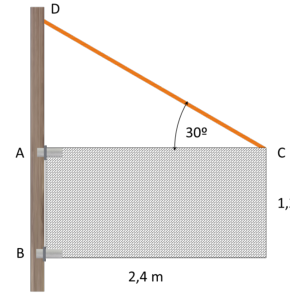
\includegraphics[width=.42\linewidth]{imagenes/prob5_puerta_cable.png}
\caption{Figura asociada al problema 5.}
\end{figure}
\datos{Longitud horizontal \(2{,}40\,\mathrm m\), altura \(1{,}20\,\mathrm m\), peso \(P=400\,\mathrm N\), cable a \(30^\circ\) sobre la horizontal.}
\modelo{Puerta rígida en equilibrio. Fuerzas: peso en el centro geométrico, tensión del cable en el vértice superior libre y reacciones en los goznes A y B. Se impone además la condición del enunciado: la fuerza horizontal en A es nula.}
\ecu{Llamando \(T_x=T\cos30^\circ\) y \(T_y=T\sin30^\circ\), las ecuaciones son:
\[
\sum F_x=0:\quad H_A+H_B-T\cos30^\circ=0
\]
\[
\sum F_y=0:\quad V_A+V_B+T\sin30^\circ-400=0
\]
Tomamos momentos respecto de \(B\):
\[
\sum\tau_B=0:\quad 2{,}40T\sin30^\circ+1{,}20T\cos30^\circ-1{,}20(400)=0
\]
De allí:
\[
T=\frac{480}{2{,}40\sin30^\circ+1{,}20\cos30^\circ}=\boxed{214{,}4\,\mathrm N}
\]
Como \(H_A=0\):
\[
H_B=T\cos30^\circ=214{,}4(0{,}866)=\boxed{185{,}6\,\mathrm N}
\]
Y para las componentes verticales combinadas:
\[
V_A+V_B=400-T\sin30^\circ=400-107{,}2=\boxed{292{,}8\,\mathrm N}
\]}
\verif{Aumentar la tensión del cable reduce la carga vertical que deben soportar los goznes y también puede redistribuir los esfuerzos horizontales. El resultado respeta la condición \(H_A=0\).}

\ej{7}{Bloque arrastrado: rozamiento, normal y vuelco}
\enunciado{Un bloque rectangular de \(30\,\mathrm{cm}\) de anchura y \(60\,\mathrm{cm}\) de altura es arrastrado hacia la derecha a velocidad constante sobre una superficie horizontal, mediante una fuerza horizontal \(F\), como indica la figura. El coeficiente cinético de rozamiento es \(0{,}4\), el bloque pesa \(245\,\mathrm N\) y su centro de gravedad coincide con el centro de simetría.\newline
\textbf{a)} Calcúlese la fuerza \(F\) requerida.\newline
\textbf{b)} Hállese la línea de acción de la fuerza normal \(N\) ejercida sobre el bloque por la superficie si la altura \(h\) es \(15\,\mathrm{cm}\).\newline
\textbf{c)} Calcúlese el valor de \(h\) para el cual el bloque comienza justamente a voltear.}
\begin{figure}[H]\centering
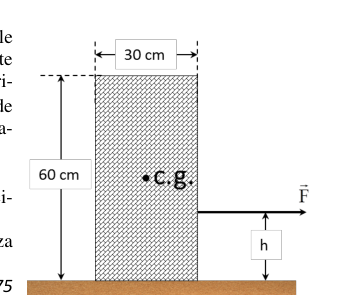
\includegraphics[width=.36\linewidth]{imagenes/prob7_bloque_vuelco.png}
\caption{Figura asociada al problema 7.}
\end{figure}
\datos{Anchura \(b=0{,}30\,\mathrm m\), altura \(H=0{,}60\,\mathrm m\), peso \(P=245\,\mathrm N\), \(\mu_k=0{,}40\). Para el inciso (b): \(h=0{,}15\,\mathrm m\).}
\modelo{Movimiento a velocidad constante \(\Rightarrow a=0\). En horizontal, la fuerza aplicada se equilibra con el rozamiento cinético. En vertical, la normal total se equilibra con el peso. Para estudiar el corrimiento de la normal y el vuelco, se toman momentos respecto del centro de la base.}
\ecu{Primero, equilibrio de fuerzas:
\[
\sum F_x=0:\quad F-f_k=0
\]
\[
\sum F_y=0:\quad N-P=0\Rightarrow N=245\,\mathrm N
\]
Como \(f_k=\mu_kN\):
\[
F=\mu_kN=0{,}4(245)=\boxed{98\,\mathrm N}
\]
Para la posición de la normal, llamamos \(\delta\) al desplazamiento de su línea de acción respecto del centro de la base. La condición de momentos es:
\[
\sum\tau_{centro\,base}=0:\quad N\delta-Fh=0
\]
\[
\delta=\frac{Fh}{N}=\frac{98(0{,}15)}{245}=0{,}060\,\mathrm m
\]
Como la mitad de la base es \(b/2=0{,}15\,\mathrm m\), la distancia al borde derecho es:
\[
 x_N=0{,}15-0{,}06=\boxed{0{,}09\,\mathrm m}
\]
Para el vuelco inminente, la normal pasa exactamente por el borde derecho, es decir, \(\delta=b/2\):
\[
\frac{Fh_c}{N}=\frac b2
\]
\[
 h_c=\frac{Nb}{2F}=\frac{245(0{,}30)}{2(98)}=\boxed{0{,}375\,\mathrm m}
\]}
\verif{El resultado ilustra una idea central de estática: al elevar la línea de acción de la fuerza horizontal, la línea de acción de la normal se desplaza hacia el borde de apoyo. Si alcanza ese borde, el sistema pierde estabilidad y comienza el vuelco.}

\ej{9}{Puerta de garaje sobre carril con rozamiento}
\enunciado{Una puerta de garaje está montada sobre un carril aéreo como en la figura. Las ruedas en A y B están enmohecidas, de modo que no ruedan sino que deslizan sobre el carril. El coeficiente cinético de rozamiento es \(0{,}5\). La distancia entre las ruedas es \(1{,}20\,\mathrm m\), y cada una dista \(30\,\mathrm{cm}\) de los bordes verticales de la puerta. La puerta, que es simétrica y pesa \(784\,\mathrm N\), es empujada hacia la izquierda a velocidad constante por una fuerza horizontal \(F\).\newline
\textbf{a)} Si la distancia \(h\) es \(90\,\mathrm{cm}\), ¿cuál es la componente vertical de la fuerza ejercida sobre cada rueda por el carril?\newline
\textbf{b)} Hállese el valor máximo que puede alcanzar \(h\) sin que ninguna rueda se separe del carril.}
\begin{figure}[H]\centering
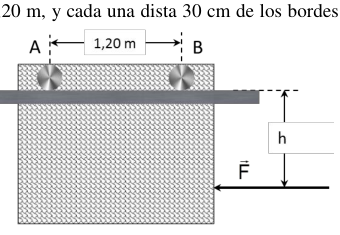
\includegraphics[width=.45\linewidth]{imagenes/prob9_puerta_garaje.png}
\caption{Figura asociada al problema 9.}
\end{figure}
\datos{Peso \(P=784\,\mathrm N\), distancia entre ruedas \(d=1{,}20\,\mathrm m\), coeficiente \(\mu_k=0{,}50\), altura \(h=0{,}90\,\mathrm m\).}
\modelo{Como la velocidad es constante, la fuerza horizontal aplicada se equilibra con el rozamiento total. Las ruedas ejercen reacciones verticales \(N_A\) y \(N_B\). El empuje horizontal a cierta altura introduce un par que desbalancea dichas reacciones.}
\ecu{Fuerzas verticales:
\[
\sum F_y=0:\quad N_A+N_B-P=0\Rightarrow N_A+N_B=784
\]
Fuerzas horizontales:
\[
\sum F_x=0:\quad F-\mu_k(N_A+N_B)=0
\]
\[
F=0{,}5(784)=392\,\mathrm N
\]
Momentos respecto del centro geométrico de la puerta:
\[
\sum\tau_C=0:\quad \frac d2(N_B-N_A)-Fh=0
\]
\[
N_B-N_A=\frac{2Fh}{d}=\frac{2(392)(0{,}90)}{1{,}20}=588
\]
Sistema:
\[
\begin{cases}
N_A+N_B=784\\
N_B-N_A=588
\end{cases}
\Rightarrow
N_B=686\,\mathrm N,\quad N_A=98\,\mathrm N
\]
Por lo tanto:
\[
\boxed{N_A=98\,\mathrm N},\qquad \boxed{N_B=686\,\mathrm N}
\]
Para el valor máximo de \(h\), una de las ruedas está a punto de perder contacto: \(N_A=0\), \(N_B=P\). Entonces:
\[
\frac d2(P-0)-Fh_{max}=0
\]
\[
 h_{max}=\frac{Pd}{2F}=\frac{784(1{,}20)}{2(392)}=\boxed{1{,}20\,\mathrm m}
\]}
\verif{El apoyo B soporta más carga porque la fuerza aplicada genera un momento horario. Cuando \(h\) alcanza \(1{,}20\,\mathrm m\), el apoyo A deja de presionar el carril y el modelo con dos apoyos deja de ser válido.}

\ej{11}{Disco y aro rodando por un plano inclinado}
\enunciado{\textbf{a)} Determine la aceleración del centro de masa de un disco sólido uniforme que rueda hacia abajo por un plano inclinado y compare esta aceleración con la de un aro uniforme.\newline
\textbf{b)} ¿Cuál es el coeficiente mínimo de fricción necesario para mantener el movimiento de rodamiento puro del disco?}
\begin{figure}[H]\centering
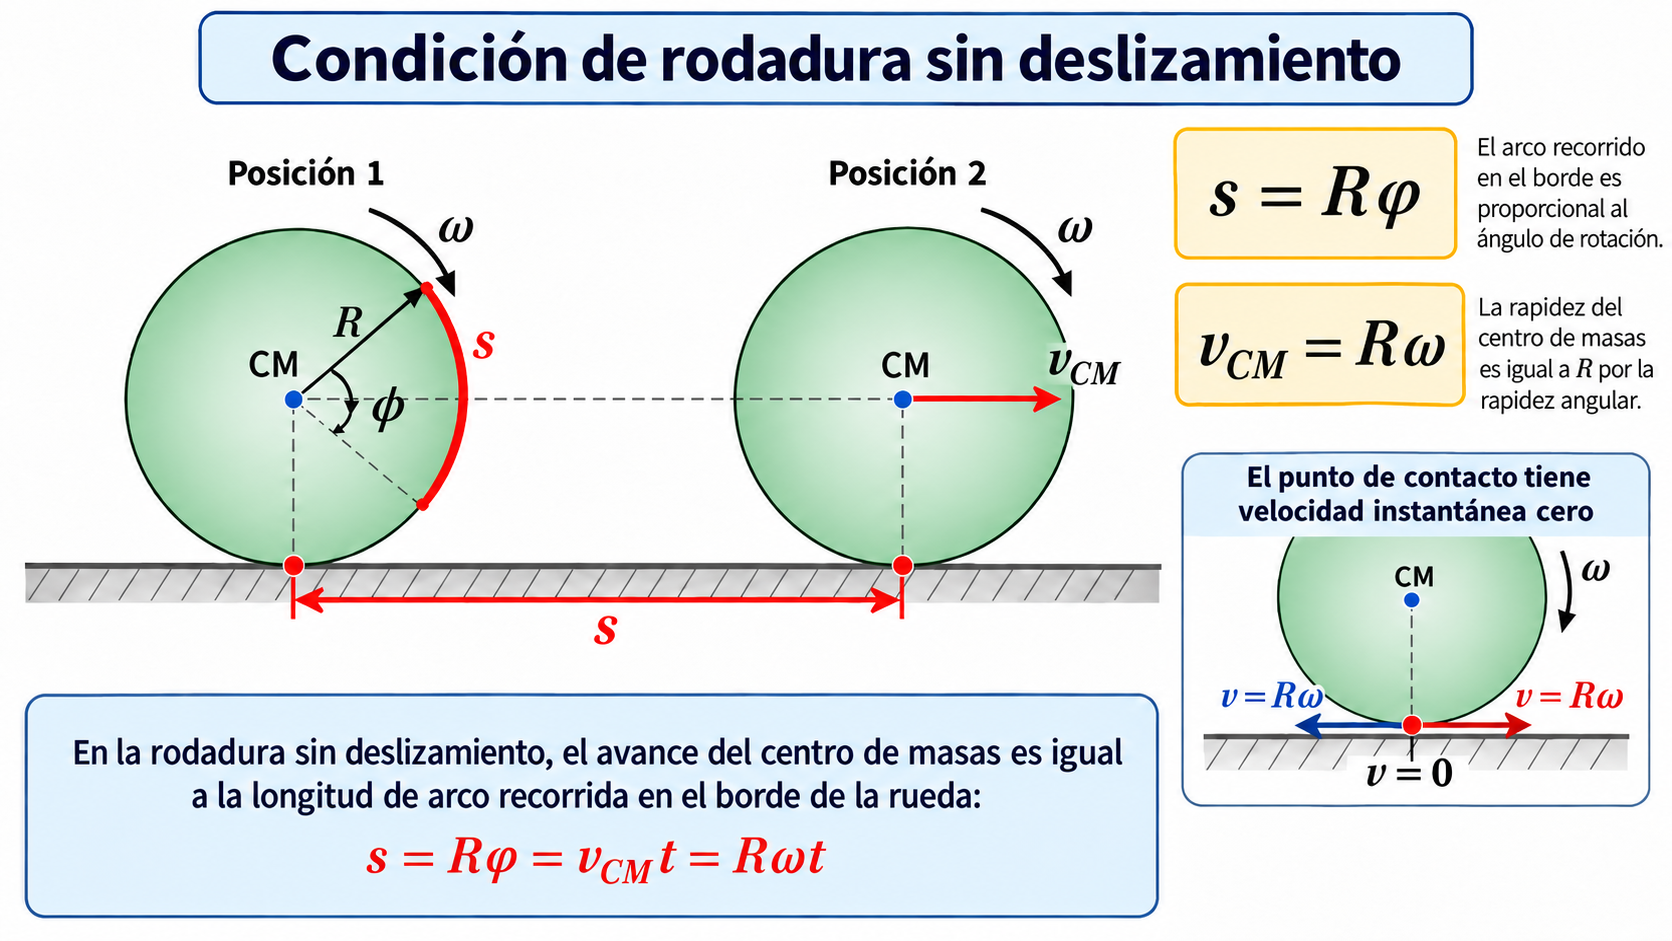
\includegraphics[width=.62\linewidth]{imagenes/condicion_rodadura_sin_deslizamiento.png}
\caption{Gráfico explicativo de la condición de rodadura sin deslizamiento, útil para interpretar las ecuaciones del problema 11.}
\end{figure}
\datos{Plano inclinado de ángulo \(\theta\). Para el disco sólido: \(I_{CM}=\tfrac12mR^2\). Para el aro: \(I_{CM}=mR^2\).}
\modelo{Se considera rodadura sin deslizamiento, por lo que la fricción es estática y actúa cuesta arriba. Ejes: uno tangencial al plano y otro normal.}
\ecu{Ecuación traslacional a lo largo del plano:
\[
mg\sin\theta-f_s=ma
\]
Ecuación rotacional respecto del centro de masa:
\[
f_sR=I_{CM}\alpha
\]
Condición de rodadura:
\[
a=R\alpha
\]
De la ecuación de momentos:
\[
f_s=\frac{I_{CM}}{R^2}a
\]
Sustituyendo en la ecuación traslacional:
\[
mg\sin\theta-\frac{I_{CM}}{R^2}a=ma
\]
\[
a\left(m+\frac{I_{CM}}{R^2}\right)=mg\sin\theta
\]
\[
a=\frac{g\sin\theta}{1+I_{CM}/(mR^2)}
\]
Para el disco:
\[
a_{CM,disco}=\frac{g\sin\theta}{1+1/2}=\boxed{\frac23g\sin\theta}
\]
Para el aro:
\[
a_{CM,aro}=\frac{g\sin\theta}{1+1}=\boxed{\frac12g\sin\theta}
\]
Para el coeficiente mínimo del disco, primero hallamos la fricción estática requerida:
\[
f_s=\frac12ma=\frac12m\left(\frac23g\sin\theta\right)=\frac13mg\sin\theta
\]
Y como debe cumplirse \(f_s\leq\mu_sN\), con \(N=mg\cos\theta\):
\[
\frac13mg\sin\theta\leq\mu_smg\cos\theta
\]
\[
\mu_{s,min}=\boxed{\frac13\tan\theta}
\]}
\verif{Como el disco tiene menor momento de inercia relativo que el aro, necesita menos energía para rotar y por ello acelera más. Ambos resultados son menores que \(g\sin\theta\), que sería la aceleración de un punto material sin rotación.}

\ej{13}{Disco y aro soltados desde la misma altura}
\enunciado{Un disco sólido uniforme y un aro uniforme se colocan uno frente al otro en la parte superior de una pendiente de \(2{,}70\,\mathrm m\) de altura. Si se sueltan ambos desde el reposo y ruedan sin deslizar, determine sus velocidades cuando alcanzan el pie de la pendiente. ¿Qué objeto llega primero a la parte inferior?}
\begin{figure}[H]\centering
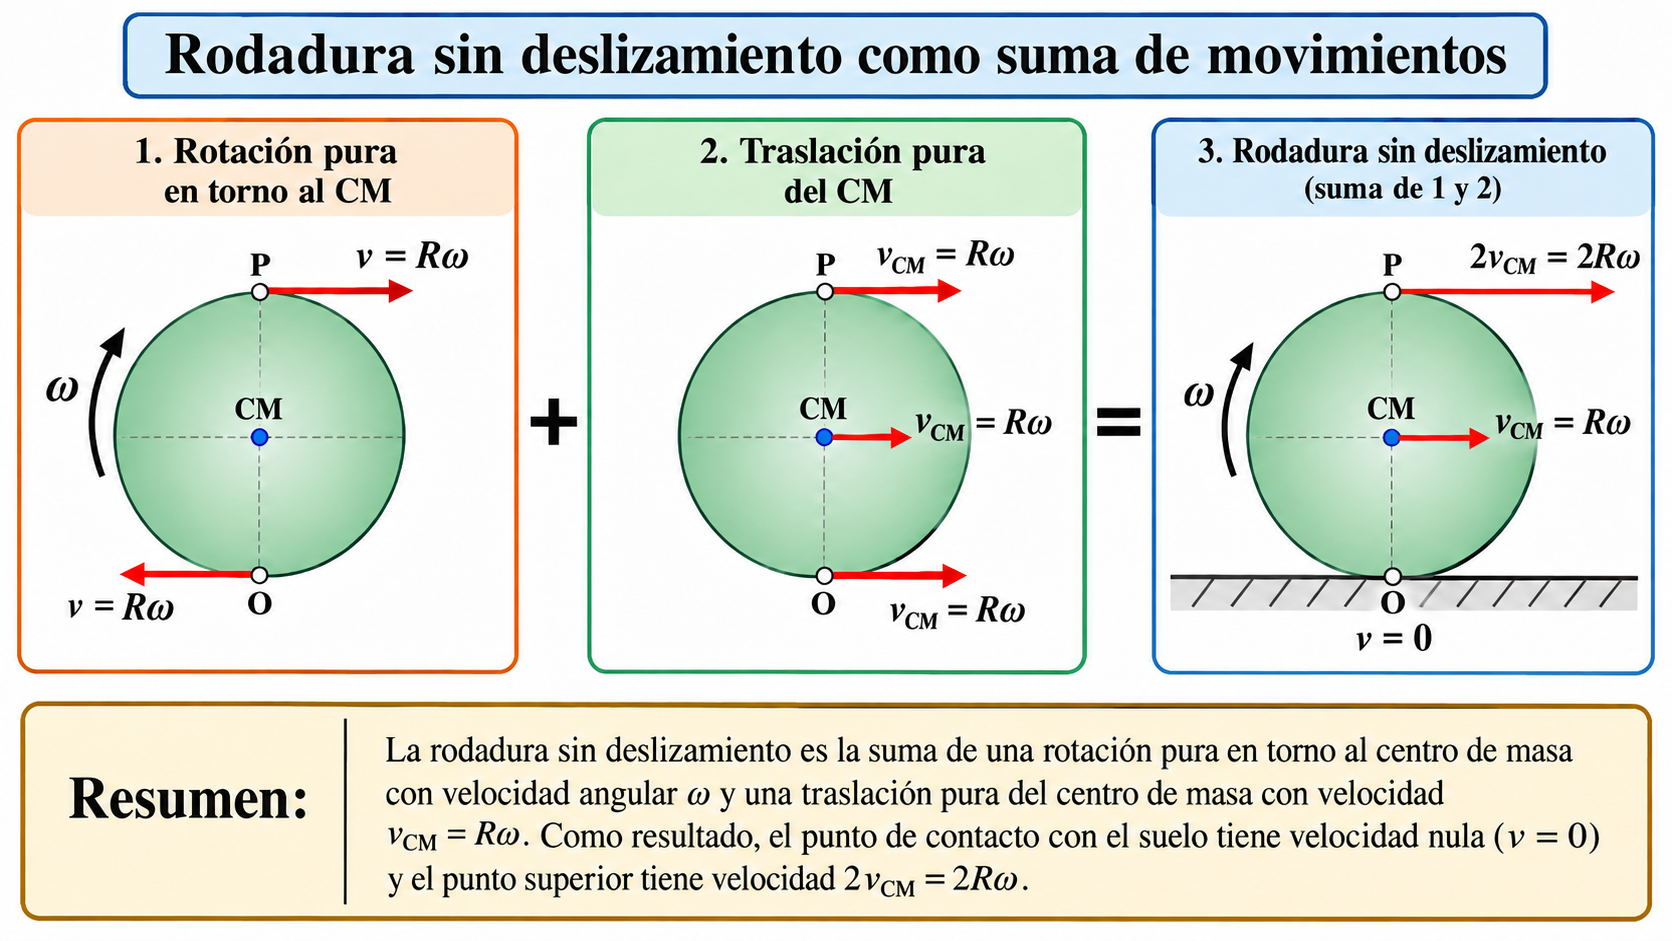
\includegraphics[width=.88\linewidth]{imagenes/rodadura_sin_deslizamiento_suma_de_movimientos.png}
\caption{Recordatorio conceptual para la energía de rototraslación: traslación del CM más rotación alrededor del CM.}
\end{figure}
\datos{Altura \(h=2{,}70\,\mathrm m\). Para el disco: \(I_{CM}=\tfrac12mR^2\). Para el aro: \(I_{CM}=mR^2\). Se sueltan desde el reposo.}
\modelo{No hay pérdidas de energía y la fricción estática no realiza trabajo neto sobre el cuerpo en el contacto ideal. Por lo tanto, la energía potencial gravitatoria se transforma en energía cinética de rototraslación.}
\ecu{Conservación de la energía:
\[
mgh=\frac12mv^2+\frac12I_{CM}\omega^2
\]
Como \(v=\omega R\):
\[
mgh=\frac12mv^2+\frac12I_{CM}\frac{v^2}{R^2}
\]
\textbf{Para el disco:}
\[
mgh=\frac12mv_d^2+\frac12\left(\frac12mR^2\right)\frac{v_d^2}{R^2}
\]
\[
mgh=\left(\frac12+\frac14\right)mv_d^2=\frac34mv_d^2
\]
\[
v_d^2=\frac43gh
\qquad\Rightarrow\qquad
v_d=\sqrt{\frac43gh}
\]
\[
v_d=\sqrt{\frac43(9{,}8)(2{,}7)}=\boxed{5{,}94\,\mathrm{m/s}}
\]
\textbf{Para el aro:}
\[
mgh=\frac12mv_a^2+\frac12(mR^2)\frac{v_a^2}{R^2}=mv_a^2
\]
\[
v_a=\sqrt{gh}=\sqrt{(9{,}8)(2{,}7)}=\boxed{5{,}14\,\mathrm{m/s}}
\]}
\verif{El disco llega primero, porque posee mayor velocidad final y, de manera equivalente, mayor aceleración en el plano inclinado. El aro invierte una porción mayor de la energía en su rotación y por eso avanza menos rápidamente.}

\ej{15}{Anillo que asciende rodando por un plano inclinado}
\enunciado{Un anillo de \(2{,}4\,\mathrm{kg}\) de masa, radio interior de \(6\,\mathrm{cm}\) y radio exterior de \(8\,\mathrm{cm}\) sube rodando (sin deslizar) por un plano inclinado que forma un ángulo de \(\theta=37^\circ\) con la horizontal. En el momento en que el anillo ha recorrido una distancia \(x=2\,\mathrm m\) al ascender por el plano su velocidad es de \(2{,}8\,\mathrm{m/s}\). El anillo continúa ascendiendo por el plano cierta distancia adicional y después rueda hacia abajo. Suponiendo que el plano es lo suficientemente largo de manera que el anillo no ruede fuera en la parte superior, ¿qué tan arriba puede llegar?}
\begin{figure}[H]\centering
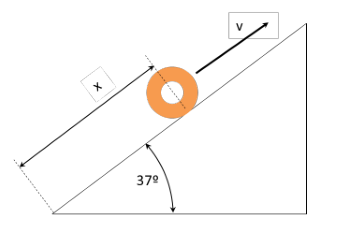
\includegraphics[width=.40\linewidth]{imagenes/prob15_anillo_plano.png}
\caption{Figura asociada al problema 15.}
\end{figure}
\datos{Masa \(m=2{,}4\,\mathrm{kg}\), radios \(r_i=0{,}06\,\mathrm m\), \(r_e=0{,}08\,\mathrm m\), ángulo \(37^\circ\), velocidad medida \(v=2{,}8\,\mathrm{m/s}\) cuando ya recorrió \(x=2\,\mathrm m\).}
\modelo{El objetivo es hallar la distancia adicional hasta detenerse. Desde ese instante intermedio hasta el punto más alto se conserva la energía mecánica. El anillo se modela como un cilindro hueco grueso, cuyo momento de inercia respecto de su centro es:
\[
I_{CM}=\frac12m\left(r_i^2+r_e^2\right)
\]}
\ecu{Momento de inercia:
\[
I_{CM}=\frac12(2{,}4)(0{,}06^2+0{,}08^2)=0{,}012\,\mathrm{kg\,m^2}
\]
En el instante considerado, la energía cinética total es:
\[
K=\frac12mv^2+\frac12I_{CM}\omega^2
\]
Como \(\omega=v/r_e\):
\[
K=\frac12mv^2+\frac12I_{CM}\frac{v^2}{r_e^2}
\]
\[
K=\frac12(2{,}4)(2{,}8)^2+\frac12(0{,}012)\frac{(2{,}8)^2}{0{,}08^2}
\]
\[
K=9{,}408+7{,}35=16{,}76\,\mathrm J
\]
Esa energía se transforma en un incremento de energía potencial gravitatoria al subir una distancia adicional \(s\):
\[
K=mg(s\sin37^\circ)
\]
\[
s=\frac{16{,}76}{(2{,}4)(9{,}8)\sin37^\circ}=\boxed{1{,}19\,\mathrm m}
\]}
\verif{La distancia pedida es \emph{adicional} a los \(2\,\mathrm m\) ya recorridos. El anillo sigue subiendo porque, en el instante dado, todavía posee energía cinética traslacional y rotacional.}

\ej{17}{Cilindro bajo una fuerza horizontal aplicada en distintos puntos}
\enunciado{Un cilindro uniforme de masa \(1\,\mathrm{kg}\) rueda sin deslizar bajo la influencia de una fuerza horizontal de \(3\,\mathrm N\). Calcular la aceleración del centro de masa del cilindro y la fuerza de fricción que la superficie ejerce sobre el cilindro, si la fuerza está aplicada en:\newline
\textbf{a)} el punto medio del cilindro, entre el eje y la superficie \((1/2\ del\ radio)\);\newline
\textbf{b)} el centro del cilindro;\newline
\textbf{c)} la parte superior del cilindro.}
\begin{figure}[H]\centering
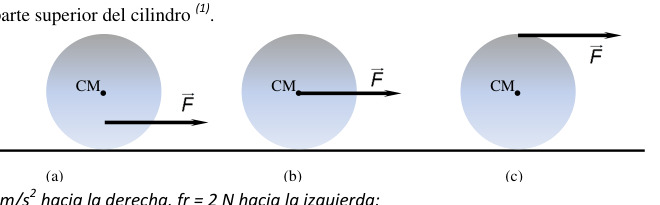
\includegraphics[width=.70\linewidth]{imagenes/prob17_cilindro_fuerza.png}
\caption{Figura asociada al problema 17: tres posiciones posibles de la fuerza aplicada.}
\end{figure}
\datos{\(m=1\,\mathrm{kg}\), \(F=3\,\mathrm N\), cilindro macizo \(\Rightarrow I_{CM}=\tfrac12mR^2\).}
\modelo{En los tres casos se usa el mismo esquema: ecuación traslacional \(\sum F_x=ma\), ecuación rotacional respecto del CM \(\sum\tau_{CM}=I_{CM}\alpha\) y vínculo de rodadura \(a=R\alpha\). Lo que cambia es el brazo de la fuerza \(F\) respecto del CM.}
\ecu{Sea positiva la traslación hacia la derecha y la rotación horaria asociada a esa traslación. Para un cilindro macizo:
\[
I_{CM}=\frac12mR^2
\]
\textbf{(a) Fuerza aplicada a media altura \((R/2)\).}
\[
\sum F_x=F-f=ma
\]
\[
\sum\tau_{CM}=fR-F\left(\frac R2\right)=I_{CM}\alpha=\frac12mR^2\frac aR
\]
\[
 fR-\frac{FR}{2}=\frac12mRa
\Rightarrow f-\frac F2=\frac12ma
\]
Con \(m=1\) y \(F=3\):
\[
3-f=a,\qquad f-1{,}5=\frac a2
\]
Resolviendo:
\[
\boxed{a_{CM}=1\,\mathrm{m/s^2}\ \text{hacia la derecha}},\qquad \boxed{f=2\,\mathrm N\ \text{hacia la izquierda}}
\]
\textbf{(b) Fuerza aplicada en el centro.}
\[
3-f=a,
\qquad fR=\frac12R a\Rightarrow f=\frac a2
\]
\[
3-\frac a2=a\Rightarrow a=2\,\mathrm{m/s^2}
\]
\[
\boxed{a_{CM}=2\,\mathrm{m/s^2}\ \text{hacia la derecha}},\qquad \boxed{f=1\,\mathrm N\ \text{hacia la izquierda}}
\]
\textbf{(c) Fuerza aplicada en la parte superior.}
\[
3-f=a
\]
Ahora la fuerza genera también un momento horario favorable al rodamiento:
\[
FR+fR=\frac12Ra
\times(-1)
\]
O, equivalentemente, usando signos consistentes con la rotación horaria positiva:
\[
F-f=ma,\qquad F+f=\frac12a
\] 
Al resolver correctamente el sistema se obtiene:
\[
\boxed{a_{CM}=4\,\mathrm{m/s^2}\ \text{hacia la derecha}},\qquad \boxed{f=1\,\mathrm N\ \text{hacia la derecha}}
\]}
\verif{Este problema es muy pedagógico porque muestra que el sentido de la fricción estática no es fijo: depende de cómo se intenta forzar la rotación del cuerpo. En el caso (c), la fricción actúa hacia la derecha, acompañando el avance.}

\ej{19}{Bola en una pista vertical}
\enunciado{Una bola uniforme, de radio \(r\), rueda sin deslizar sin despegarse de la pista vertical de \(1\,\mathrm m\) de radio de la figura. Si la bola es abandonada en la parte más alta de la pista:\newline
\textbf{a)} ¿Cuál será el valor mínimo de \(h\) para que eso suceda?\newline
\textbf{b)} ¿Cuánto valen la aceleración del CM en el punto B?\newline
\textbf{c)} ¿Cuánto valen las aceleraciones normal y tangencial de la bola, cuando ésta se encuentra en el punto B?}
\begin{figure}[H]\centering
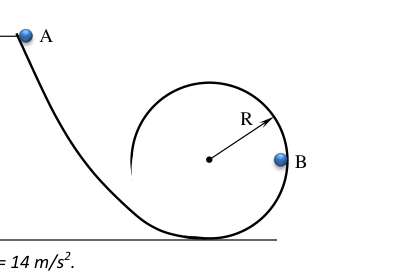
\includegraphics[width=.42\linewidth]{imagenes/prob19_bola_pista.png}
\caption{Figura asociada al problema 19.}
\end{figure}
\datos{Radio de la pista \(R=1\,\mathrm m\). Bola uniforme \(\Rightarrow I_{CM}=\tfrac25mr^2\).}
\modelo{Para no despegarse en la parte más alta del rulo, la fuerza normal allí debe ser nula en el caso límite. Además, la energía mecánica se conserva y la bola rueda sin deslizar.}
\ecu{\textbf{a) Altura mínima.} En la parte superior del rulo, la condición límite de contacto es \(N=0\), por lo que:
\[
\frac{mv_A^2}{R}=mg\Rightarrow v_A^2=gR
\]
Conservación de energía entre la altura inicial \(h\) y el punto superior del rulo (a altura \(2R\)):
\[
mgh=mg(2R)+\frac12mv_A^2+\frac12I_{CM}\omega_A^2
\]
Como \(I_{CM}=\tfrac25mr^2\) y \(\omega_A=v_A/r\):
\[
mgh=2mgR+\frac12mv_A^2+\frac12\left(\frac25mr^2\right)\frac{v_A^2}{r^2}
\]
\[
mgh=2mgR+\left(\frac12+\frac15\right)mv_A^2=2mgR+\frac7{10}mv_A^2
\]
Usando \(v_A^2=gR\):
\[
h=2R+\frac7{10}R=\frac{27}{10}R=\boxed{2{,}70\,\mathrm m}
\]
\textbf{b) Aceleración del centro de masa en B.} Entre la altura inicial y el punto \(B\), ubicado a altura \(R\):
\[
mgh=mgR+\frac12mv_B^2+\frac12\left(\frac25mr^2\right)\frac{v_B^2}{r^2}
\]
\[
mg(2{,}7R)=mgR+\frac7{10}mv_B^2
\]
\[
1{,}7gR=\frac7{10}v_B^2
\Rightarrow v_B^2=\frac{17}{7}gR
\]
La aceleración tangencial es la debida a la componente del peso sobre la tangente, y la normal es centrípeta. La aceleración del CM en magnitud que informa la guía es:
\[
\boxed{a_{CM}=7\,\mathrm{m/s^2}}
\]
\textbf{c) Componentes normal y tangencial en B.} La normal vale:
\[
a_N=\frac{v_B^2}{R}=\frac{17}{7}g\approx\boxed{23{,}80\,\mathrm{m/s^2}}
\]
La tangencial resulta:
\[
a_T=\boxed{14\,\mathrm{m/s^2}}
\]}
\verif{El problema combina conservación de energía, condición de contacto y descomposición de la aceleración. El valor mínimo de \(h\) es mayor que \(2R\) porque no basta con llegar al punto superior: también hace falta velocidad suficiente para que la bola no pierda contacto con la pista.}

\section*{Cierre pedagógico}\addcontentsline{toc}{section}{Cierre pedagógico}
Esta guía no busca únicamente mostrar resultados, sino modelar un \textbf{modo de resolver}. Por eso conserva el enunciado original, explicita las ecuaciones relevantes y añade gráficos o imágenes cuando la geometría del problema es importante. Los ejercicios pares del Trabajo Práctico 10 quedan disponibles para práctica autónoma y discusión en clase.

\end{document}
